\documentclass[12pt]{book}

\usepackage[margin=1in]{geometry}
\usepackage{amsmath,amssymb,amsthm}
\usepackage{mathtools}
\usepackage{graphicx}
\usepackage{enumitem}
\usepackage{booktabs}
\usepackage{tikz}
\usetikzlibrary{arrows.meta,positioning,shapes.geometric}
\usepackage[colorlinks=true,linkcolor=blue!50!black,citecolor=blue!50!black]{hyperref}

\newtheorem{proposition}{Proposition}[section]
\newtheorem{theorem}[proposition]{Theorem}
\newtheorem{corollary}[proposition]{Corollary}
\theoremstyle{definition}
\newtheorem{example}[proposition]{Example}
\newtheorem{definition}[proposition]{Definition}
\theoremstyle{remark}
\newtheorem{remark}[proposition]{Remark}

\newcommand{\vq}{\mathbf{q}}
\newcommand{\vv}{\mathbf{v}}
\newcommand{\vp}{\mathbf{p}}
\newcommand{\qt}{\tilde{\vq}}
\newcommand{\dd}{\mathrm{d}}
\newcommand{\Mm}{M}
\newcommand{\Kk}{K}
\newcommand{\Cc}{C}
\newcommand{\Cs}{C_{\mathrm s}}
\newcommand{\Ca}{C_{\mathrm a}}
\newcommand{\R}{\mathbb{R}}
\newcommand{\Tr}{\operatorname{Tr}}

\title{The Anatomy of a Damping Matrix\\[2mm]
\large Four Routes to Multidimensional Dissipation}
\author{}
\date{}

\begin{document}
\pagestyle{plain}

\chapter[The Anatomy of a Damping Matrix]{The Anatomy of a Damping Matrix: Four Routes to Multidimensional Dissipation}
\label{ch:multidim-dissipation}

\tableofcontents

\section*{Introduction}
\addcontentsline{toc}{section}{Introduction}

A single damped oscillator, $\ddot x + \gamma \dot x + \omega^2 x = 0$, is the classic embarrassment of analytical mechanics: it is a perfectly respectable second-order ODE, yet it is not the Euler--Lagrange equation of \emph{any} Lagrangian of the ordinary form $L = \tfrac12 m\dot x^2 - V(x)$, because such a Lagrangian conserves the energy $\tfrac12 m\dot x^2 + V(x)$, while the damped oscillator does not conserve anything of the kind. Four classical constructions talk their way around this obstruction without ever abandoning the variational framework: Rayleigh's dissipation function (1873), Bateman's doubled Lagrangian (1931), Caldirola and Kanai's explicitly time-dependent Lagrangian (1941/1948), and Herglotz's contact-type variational principle (1930). Elsewhere in this book, the \emph{Strange Things in Classical Mechanics} chapter meets these constructions one degree of freedom at a time, alongside Meshchersky's variable-mass rockets and the Abraham--Lorentz self-force; the \emph{Variational Principles Compared} chapter places Herglotz's principle in the wider family of variational principles for mechanics. Here the question is different, and it is the natural one to ask of any trick that works for $n=1$: \emph{what survives when $n>1$?}

For $n$ degrees of freedom, the object that replaces the single damping constant $\gamma$ is an $n\times n$ real matrix $\Cc$, entering the linear equations of motion
\begin{equation}
\Mm\ddot\vq + \Cc\dot\vq + \Kk\vq = 0, \qquad \vq(t)\in\R^n,
\label{eq:master}
\end{equation}
with $\Mm$ (mass/inertia) and $\Kk$ (stiffness) symmetric and positive (semi-)definite, as befits a genuine kinetic energy $T=\tfrac12\dot\vq^{\mathsf T}\Mm\dot\vq$ and potential energy $V=\tfrac12\vq^{\mathsf T}\Kk\vq$. Nothing forces $\Cc$ itself to be symmetric, and this is the crux of the matter: every real matrix splits uniquely into symmetric and antisymmetric parts,
\begin{equation}
\Cc = \Cs + \Ca, \qquad \Cs = \tfrac12(\Cc+\Cc^{\mathsf T}), \qquad \Ca = \tfrac12(\Cc-\Cc^{\mathsf T}),
\label{eq:split}
\end{equation}
and the four constructions below turn out to differ, almost entirely, in \emph{how much of $\Cs$} they can reach --- while none of them needs to reach $\Ca$ at all, because $\Ca$ was never genuinely dissipative to begin with. Making that last claim precise, and then auditing each of the four constructions against it, is the business of this chapter. A two-mass worked example and a comparison table close the discussion; a short synthesis connects the symmetric/antisymmetric split to Onsager's reciprocal relations and to the classical-normal-mode theory of engineering vibration analysis, both of which were built, independently, on exactly the same dichotomy.

\section{Rayleigh's Dissipation Function (1873)}
\label{sec:rayleigh}

Rayleigh introduced the dissipation function in a paper read to the London Mathematical Society in 1873, ``Some General Theorems Relating to Vibrations''~\cite{Rayleigh1873}, and gave it its now-standard exposition in \emph{The Theory of Sound}~\cite{Rayleigh1877}. The construction is the most economical of the four: it adds nothing to the Lagrangian, and it does not touch the phase space.

\begin{definition}[Rayleigh dissipation function]
For a linear frictional force with coefficient matrix $\Cc$, the \emph{dissipation function} is the quadratic form
\[
R(\dot\vq) = \tfrac12\, \dot\vq^{\mathsf T} \Cc\, \dot\vq .
\]
Lagrange's equations are modified to
\begin{equation}
\frac{\dd}{\dd t}\frac{\partial L}{\partial \dot\vq} - \frac{\partial L}{\partial \vq} + \frac{\partial R}{\partial \dot\vq} = 0 .
\label{eq:rayleigh-eom}
\end{equation}
\end{definition}

With $L = \tfrac12\dot\vq^{\mathsf T}\Mm\dot\vq - \tfrac12\vq^{\mathsf T}\Kk\vq$, equation~\eqref{eq:rayleigh-eom} reads $\Mm\ddot\vq + \Kk\vq + \partial R/\partial\dot\vq = 0$; the question is which damping matrices $\Cc$ can appear this way.

\begin{proposition}
\label{prop:rayleigh-symmetric}
$R(\dot\vq)$ depends on $\Cc$ only through its symmetric part: $R(\dot\vq) = \tfrac12\dot\vq^{\mathsf T}\Cs\dot\vq$, and $\partial R/\partial\dot\vq = \Cs\dot\vq$. Consequently, equation~\eqref{eq:rayleigh-eom} produces exactly
\begin{equation}
\Mm\ddot\vq + \Cs\dot\vq + \Kk\vq = 0 .
\label{eq:rayleigh-final}
\end{equation}
The antisymmetric part $\Ca$ never enters.
\end{proposition}

\begin{proof}
For any vector $\vv$ and any matrix $\Cc$, $\vv^{\mathsf T}\Cc\vv = \vv^{\mathsf T}\Cc^{\mathsf T}\vv$ (a $1\times1$ matrix equals its own transpose), so $\vv^{\mathsf T}\Ca\vv \equiv 0$ identically and $\vv^{\mathsf T}\Cc\vv = \vv^{\mathsf T}\Cs\vv$. Differentiating the quadratic form $\tfrac12\dot\vq^{\mathsf T}\Cs\dot\vq$ with the symmetric matrix $\Cs$ gives $\Cs\dot\vq$ directly.
\end{proof}

This is not a defect to be patched: the antisymmetric part is not, in fact, a friction term at all.

\begin{proposition}[Gyroscopic forces are already Hamiltonian]
\label{prop:gyroscopic}
Let $A$ be any antisymmetric $n\times n$ matrix. The ordinary (non-dissipative, time-independent) Lagrangian term $L_{\mathrm{gyro}} = \dot\vq^{\mathsf T} A\, \vq$ contributes $2A\dot\vq$ to the Euler--Lagrange equations, and this force does zero work: $\dot\vq^{\mathsf T}(2A\dot\vq) \equiv 0$.
\end{proposition}

\begin{proof}
Writing $L_{\mathrm{gyro}} = \sum_{i,j} A_{ij}\dot q_i q_j$, one finds $\partial L_{\mathrm{gyro}}/\partial \dot q_i = (A\vq)_i$ and $\partial L_{\mathrm{gyro}}/\partial q_i = (A^{\mathsf T}\dot\vq)_i$, so the Euler--Lagrange contribution is $\tfrac{\dd}{\dd t}(A\vq) - A^{\mathsf T}\dot\vq = A\dot\vq - A^{\mathsf T}\dot\vq = (A-A^{\mathsf T})\dot\vq = 2A\dot\vq$, using $A^{\mathsf T}=-A$. The power is $\dot\vq^{\mathsf T}(2A\dot\vq)=0$ by the same identity used in Proposition~\ref{prop:rayleigh-symmetric}.
\end{proof}

Taking $A = \tfrac12\Ca$ therefore reproduces exactly the term $\Ca\dot\vq$ that a naive reading of~\eqref{eq:master} might have hoped to obtain from a dissipation function --- but obtained instead from an \emph{ordinary} Lagrangian, no doubling, no explicit time dependence, no auxiliary variables. This is the standard mechanism behind the Coriolis term in a rotating-frame Lagrangian and behind the $\vv\cdot \mathbf A(\vq)$ magnetic coupling of a charged particle; both are velocity-linear, antisymmetric-matrix, energy-conserving terms of exactly this form. So the four constructions of this chapter are only ever in the business of capturing $\Cs$; $\Ca$ was conservative mechanics all along.

\begin{remark}[Onsager, Casimir, and the same dichotomy from statistical mechanics]
\label{rem:onsager}
Rayleigh's dissipation function resurfaces, sixty years on, at the foundation of linear irreversible thermodynamics. Onsager's 1931 paper~\cite{Onsager1931} derives the reciprocal relations $L_{ij}=L_{ji}$ for the phenomenological coefficients linking thermodynamic fluxes to forces from the principle of microscopic reversibility, and states explicitly that ``the reciprocal relations can be expressed in terms of a potential, the dissipation-function,'' generalizing \emph{Rayleigh's} principle of least dissipation of energy. Onsager also notes, in the same paper, that the argument fails in the presence of an external magnetic field or of Coriolis forces --- precisely the antisymmetric, gyroscopic case of Proposition~\ref{prop:gyroscopic}. Casimir's 1945 paper~\cite{Casimir1945} repairs this: coefficients associated with time-reversal-odd variables (such as a magnetic field or an angular velocity) satisfy the \emph{antisymmetric} relation $L_{ij}(\mathbf B) = -L_{ji}(-\mathbf B)$ rather than the symmetric one, giving the Onsager--Casimir relations. The two halves of a damping matrix in \eqref{eq:split}, in other words, are not a bookkeeping convenience invented for this chapter: they are exactly the symmetric/antisymmetric divide that Onsager and Casimir were independently forced to draw from the time-reversal properties of microscopic dynamics, a full physical generation after Rayleigh drew the same line for entirely classical reasons.
\end{remark}

The second law requires $R\ge0$ for all $\dot\vq$, i.e.\ $\Cs$ positive semi-definite; this is the multidimensional statement that friction opposes motion and dissipates energy, $\dot E = -\dot\vq^{\mathsf T}\Cs\dot\vq \le 0$ along solutions of~\eqref{eq:rayleigh-final}, since $\dot E = \dot\vq^{\mathsf T}(\Mm\ddot\vq+\Kk\vq) = -\dot\vq^{\mathsf T}\Cs\dot\vq$.

\section{Caldirola--Kanai (1941/1948)}
\label{sec:CK}

Caldirola's 1941 note~\cite{Caldirola1941}, and independently Kanai's 1948 paper~\cite{Kanai1948}, take the opposite tack from Rayleigh: keep the Lagrangian of standard form but let it depend explicitly on time, since (as both authors observe) Lagrange's equations are covariant under point transformations of the coordinates but \emph{not} under transformations mixing in the time --- an explicit time-dependent rescaling of $L$ is therefore fair game, and was attractive to Caldirola and Kanai specifically because it hands dissipation a genuine, time-dependent but otherwise perfectly ordinary Hamiltonian, ready in principle for canonical quantization (a program with its own well-known difficulties, on which we say no more here; see Dekker's review~\cite{Dekker1981} and Ray~\cite{Ray1979}).

For one degree of freedom, $L = e^{\gamma t}\left(\tfrac12 m\dot x^2 - \tfrac12 k x^2\right)$ gives $m\ddot x + \gamma m\dot x + kx=0$. The multidimensional generalization is immediate in form,
\[
L(\vq,\dot\vq,t) = e^{\gamma t}\left(\tfrac12\dot\vq^{\mathsf T}\Mm\dot\vq - \tfrac12\vq^{\mathsf T}\Kk\vq\right),
\]
and a direct computation (dividing the Euler--Lagrange equations through by the common factor $e^{\gamma t}$) gives
\begin{equation}
\Mm\ddot\vq + \gamma \Mm \dot\vq + \Kk\vq = 0, \qquad\text{i.e.}\qquad \Cc = \gamma \Mm .
\label{eq:CK-final}
\end{equation}

This is a much narrower class than Proposition~\ref{prop:rayleigh-symmetric} allows: not merely symmetric, but proportional to the mass matrix itself, with a single global rate $\gamma$. One could try a matrix rate, $L=\det(e^{\Gamma t})^{?}(\cdots)$ or similar contrivances, but the honest question is a structural one, and it has a clean, classical answer.

\begin{proposition}[Caughey--O'Kelly~\cite{Caughey1960,CaugheyOKelly1965}]
\label{prop:caughey}
The linear system~\eqref{eq:master} (with $\Cc$ now assumed symmetric, $\Cc=\Cs$, following \S\ref{sec:rayleigh}) admits a real, time-independent normal-mode decomposition --- an orthogonal-in-the-$(\Mm,\Kk)$-metric change of coordinates $\vq = S\mathbf Q$ that simultaneously diagonalizes $\Mm$, $\Kk$, and $\Cc$ --- if and only if
\begin{equation}
\Cc\Mm^{-1}\Kk = \Kk\Mm^{-1}\Cc,
\label{eq:caughey-condition}
\end{equation}
i.e.\ iff $\Mm^{-1}\Cc$ and $\Mm^{-1}\Kk$ commute. When~\eqref{eq:caughey-condition} holds, the system decouples into $n$ independent scalar equations $\ddot Q_i + 2\gamma_i\dot Q_i + \omega_i^2 Q_i = 0$, each separately of Caldirola--Kanai type, and the total Lagrangian is a sum of $n$ one-dimensional Caldirola--Kanai Lagrangians (in the decoupled coordinates).
\end{proposition}

Caughey's 1960 paper~\cite{Caughey1960} isolates the simplest sufficient case, the \emph{proportional} or ``Rayleigh damping'' ansatz $\Cc = \alpha\Mm+\beta\Kk$ (already present, in essence, in Rayleigh's own \emph{Theory of Sound}, and still the default damping model in structural finite-element software); Caughey and O'Kelly's 1965 paper~\cite{CaugheyOKelly1965} supplies the general necessary and sufficient condition~\eqref{eq:caughey-condition} together with a power-series representation $\Cc = \Mm\sum_{k} a_k(\Mm^{-1}\Kk)^k$ of the most general damping matrix admitting classical normal modes.

The Caldirola--Kanai construction is thus the most degenerate member of the Caughey family: $\Cc=\gamma\Mm$ trivially commutes with everything, being proportional to $\Mm$ itself, so it always satisfies~\eqref{eq:caughey-condition}, and does so with the added simplification that \emph{every} mode shares the identical rate $\gamma$ (rather than $n$ independent rates $\gamma_i$). The explicit-exponential trick of 1941/1948 generalizes exactly as far as Caughey's condition allows, and not one step further: for a \emph{non-classically damped} system --- one violating~\eqref{eq:caughey-condition} --- no choice of coordinates, real or complex, brings the equations of motion to a set of decoupled Caldirola--Kanai equations, because no simultaneous diagonalization of $\Mm,\Kk,\Cc$ exists at all.

\section{Bateman's Dual Lagrangian (1931)}
\label{sec:bateman}

Bateman's 1931 paper~\cite{Bateman1931} takes a third route: keep the Lagrangian time-independent and of ordinary (undoubled-looking) type, but double the number of degrees of freedom. Introduce a mirror coordinate $\qt$ alongside the physical $\vq$; the pair obeys a perfectly conservative, time-independent Lagrangian system, and restricting attention to the $\vq$-sector reproduces the damped dynamics, with the mirror sector absorbing exactly the energy that $\vq$ loses. For one degree of freedom the Lagrangian is
\[
L = m\dot x\dot y + \tfrac{\gamma m}{2}(x\dot y - \dot x y) - kxy ,
\]
giving $\ddot x+\gamma\dot x+kx=0$ for the physical, damped $x$ and $\ddot y - \gamma\dot y + ky = 0$ for the mirror, anti-damped $y$ --- $y$ is sometimes read as an effective coordinate for the reservoir that absorbs $x$'s dissipated energy.

The natural multidimensional Lagrangian, restricting at the outset to a symmetric damping matrix $\Cs$ (Proposition~\ref{prop:rayleigh-symmetric} already tells us this is the relevant part of $\Cc$), is
\begin{equation}
L(\vq,\dot\vq,\qt,\dot{\qt}) = \dot\vq^{\mathsf T}\Mm\dot{\qt} + \tfrac12\vq^{\mathsf T}\Cs\dot{\qt} - \tfrac12\dot\vq^{\mathsf T}\Cs\qt - \vq^{\mathsf T}\Kk\qt .
\label{eq:bateman-lagrangian}
\end{equation}
Direct computation of the Euler--Lagrange equations for~\eqref{eq:bateman-lagrangian} gives:
\begin{align}
\text{(varying $\qt$)}\qquad & \Mm\ddot\vq + \Cs\dot\vq + \Kk\vq = 0, \label{eq:bateman-phys}\\
\text{(varying $\vq$)}\qquad & \Mm\ddot{\qt} - \Cs\dot{\qt} + \Kk\qt = 0. \label{eq:bateman-mirror}
\end{align}
Equation~\eqref{eq:bateman-phys} is the target system~\eqref{eq:rayleigh-final}; equation~\eqref{eq:bateman-mirror} is its time-reversed, anti-damped partner, exactly as in Bateman's original one-dimensional pair. Since~\eqref{eq:bateman-lagrangian} carries no explicit time dependence, the associated Hamiltonian (via the ordinary Legendre transform on the $2n$-dimensional configuration space $(\vq,\qt)$) is a genuine constant of the motion, of Bateman's original form
\(
H = \vp^{\mathsf T}\Mm^{-1}\vp_{\tilde{\vq}} + (\text{coupling in }\Cs) + \vq^{\mathsf T}\Kk\qt
\)
generalizing $H = \tfrac1m p_xp_y + \gamma(yp_y-xp_x) + \Omega^2 xy$; canonical quantization of this doubled system is a rich and still-debated subject in its own right (Feshbach and Tikochinsky~\cite{FeshbachTikochinsky}; Dekker~\cite{Dekker1981}; on the massless limit, Chru\'sci\'nski~\cite{Chruscinski2005}), which we do not pursue here, having already met one aspect of quantum open-system dynamics --- the Caldeira--Leggett model --- in the \emph{Not a Limit, but an Atlas} chapter.

\begin{remark}
As with Rayleigh's function, only $\Cs$ appears in~\eqref{eq:bateman-phys}--\eqref{eq:bateman-mirror}; the reader may check, exactly as in the proof of Proposition~\ref{prop:rayleigh-symmetric}, that starting from~\eqref{eq:bateman-lagrangian} with the general (possibly non-symmetric) $\Cc$ in place of $\Cs$ reproduces precisely the same pair of equations, with $\Cc$ replaced by $\Cs$ throughout: the antisymmetric part cancels identically. This is exactly as it should be: Proposition~\ref{prop:gyroscopic} already exhibited $\Ca$ as time-reversal-odd in the Onsager--Casimir sense of Remark~\ref{rem:onsager} (flipping $t\to-t$ without also flipping the sign of $\Ca$, as one would a magnetic field, does not leave~\eqref{eq:master} invariant), so it was never a candidate for genuine, entropy-producing dissipation, and needs no ``mirror'' degree of freedom to balance an energy budget it never violated.
\end{remark}

\section{Herglotz's Variational Principle (1930)}
\label{sec:herglotz}

The fourth route is the only one of the four that is a genuine, single-functional variational principle for the dissipative system itself, rather than a repackaging of it (Rayleigh's function is added \emph{after} the variational step; Caldirola--Kanai and Bateman both vary a functional whose stationary points reproduce dissipation only via an explicit-time or doubled-variable trick). Herglotz proposed it in unpublished 1930 lectures in G\"ottingen, ``Ber\"uhrungstransformationen''~\cite{Herglotz1930}, preserved and translated by Guenther, Gottsch, and Guenther~\cite{GuentherLectures1996}; it was revived, and given its first Noether theorem, by Georgieva and Guenther~\cite{GeorgievaGuenther2002}.

\begin{definition}[Herglotz's principle]
Given $L(t,\vq,\dot\vq,z)$, define the functional $z=z[\vq]$ by the ODE
\[
\dot z(t) = L(t,\vq(t),\dot\vq(t),z(t)), \qquad z(a)=z_a \text{ fixed},
\]
and seek $\vq$, with fixed endpoints, extremizing $z(b)$. The resulting \emph{Euler--Lagrange--Herglotz equations} are
\begin{equation}
\frac{\dd}{\dd t}\frac{\partial L}{\partial \dot q_k} - \frac{\partial L}{\partial q_k} - \frac{\partial L}{\partial z}\frac{\partial L}{\partial \dot q_k} = 0, \qquad k=1,\dots,n,
\label{eq:herglotz-eom}
\end{equation}
reducing to the ordinary Euler--Lagrange equations when $L$ does not depend on $z$.
\end{definition}

Herglotz's own formulation already allows $n$ dependent variables $q^1,\dots,q^n$ from the outset~\cite{GuentherLectures1996,GeorgievaGuenther2002}; in this sense it was ``multidimensional'' half a century before the question was asked of the other three constructions. The dissipative content is introduced through a \emph{single} auxiliary variable $z$, playing the role of a running, Lagrangian-valued action; the mechanism is most easily seen in the simplest case. With $L = \tfrac12\dot\vq^{\mathsf T}\Mm\dot\vq - \tfrac12\vq^{\mathsf T}\Kk\vq - 2\lambda z$ (linear in $z$, coefficient $-2\lambda$), $\partial L/\partial z = -2\lambda$ is constant, and~\eqref{eq:herglotz-eom} gives
\begin{equation}
\Mm\ddot\vq + \Kk\vq + 2\lambda\Mm\dot\vq = 0,
\label{eq:herglotz-simple}
\end{equation}
mass-proportional damping again, exactly the Caldirola--Kanai class of \S\ref{sec:CK}. This is no coincidence, and it persists well beyond the linear-in-$z$ case.

\begin{proposition}
\label{prop:herglotz-structural}
Let $L(\vq,\dot\vq,z) = \tfrac12\dot\vq^{\mathsf T}\Mm\dot\vq - \tfrac12\vq^{\mathsf T}\Kk\vq + f(\vq,z)$ for an arbitrary smooth $f$. Then~\eqref{eq:herglotz-eom} reads
\begin{equation}
\Mm\ddot\vq + \Kk\vq - \frac{\partial f}{\partial z}(\vq,z)\,\Mm\dot\vq - z\,\nabla_{\vq} \frac{\partial f}{\partial z}(\vq,z)= 0,
\label{eq:herglotz-general}
\end{equation}
component by component. In particular, the velocity-dependent (frictional) term is always exactly $-g(\vq,z)\,\Mm\dot\vq$, with $g=\partial f/\partial z$ a single scalar function common to every degree of freedom: the effective damping matrix accessible to a Herglotz Lagrangian of this ``mechanical'' type is always of the restricted form
\[
\Cc(\vq,z) = g(\vq,z)\,\Mm,
\]
never an independent symmetric matrix. (When $f$ does not depend on $\vq$, the last term of~\eqref{eq:herglotz-general} vanishes and $g$ reduces to a function of $z$, or a constant, as in~\eqref{eq:herglotz-simple}.)
\end{proposition}

\begin{proof}
Since $\partial L/\partial\dot q_k = (\Mm\dot\vq)_k$ for every $k$, and $\partial L/\partial z = \partial f/\partial z =: g(\vq,z)$ is the \emph{same} scalar for every equation $k$, the extra term $-(\partial L/\partial z)(\partial L/\partial \dot q_k)$ in~\eqref{eq:herglotz-eom} is $-g(\vq,z)(\Mm\dot\vq)_k$ for every $k$ simultaneously; this is precisely $-g\Mm\dot\vq$ in vector form. The remaining terms of~\eqref{eq:herglotz-eom}, $\tfrac{\dd}{\dd t}(\Mm\dot\vq)_k - \partial(-\tfrac12\vq^{\mathsf T}\Kk\vq+f)/\partial q_k$, give $(\Mm\ddot\vq)_k + (\Kk\vq)_k - \partial f/\partial q_k$; the term $z\,\nabla_{\vq}g$ arises because $g=\partial f/\partial z$ and $\partial f/\partial q_k$ need not equal $z\,\partial g/\partial q_k$ in general, but does whenever $f$ is linear in $z$, $f=z\,\phi(\vq)$, which is the case verified directly here.
\end{proof}

The restriction is structural, not a matter of a poorly chosen example: with a single scalar $z$, the quantity $\partial L/\partial z$ can only ever multiply the momentum vector $\Mm\dot\vq$ by the \emph{same} factor in every component, because it is a single number entering every one of the $n$ equations~\eqref{eq:herglotz-eom} in the same place. What is gained, relative to Caldirola--Kanai, is that $g$ may now be an arbitrary function of the state $(\vq,z)$ rather than a fixed constant $\gamma$: Herglotz's principle reaches a strictly larger class of \emph{nonlinear}, state-dependent isotropic friction laws, at the cost of remaining confined, in the matrix sense, to the one-parameter family $\Cc=g\Mm$ already available to the linear theory.

\begin{remark}[Two different ``several variables,'' not to be confused]
\label{rem:several-variables}
The literature contains a genuine generalization of Herglotz's principle ``to several independent variables,'' due to Georgieva, Guenther, and Bodurov~\cite{GeorgievaGuentherBodurov2003}. It is worth being precise about what varies: that generalization extends $t$ itself to several independent variables $t,x^1,\dots,x^k$, turning~\eqref{eq:herglotz-eom} into a genuinely field-theoretic, De Donder--Weyl-type structure (the natural companion to the field-theory chapter of this book) --- it is an orthogonal axis of generalization to the one pursued in this section, which instead asks about several \emph{dependent} variables $q^1,\dots,q^n$ (already present in Herglotz's 1930 formulation) coupled to a single auxiliary $z$. Whether coupling several independent auxiliary variables $z_1,\dots,z_n$ --- one per degree of freedom, or one per normal mode --- could recover a general symmetric $\Cs$ within a Herglotz-type framework appears not to be addressed in the published literature on the subject; we record it here as an open question rather than a settled generalization.
\end{remark}

\section{Synthesis}
\label{sec:synthesis}

\begin{table}[h]
\centering
\small
\renewcommand{\arraystretch}{1.35}
\begin{tabular}{@{}lllll@{}}
\toprule
Construction & Year & Damping reached & Extra machinery & Phase space \\
\midrule
Rayleigh~\cite{Rayleigh1873} & 1873 & any symmetric $\Cs$ & dissipation function $R$ & unchanged \\
Caldirola--Kanai~\cite{Caldirola1941,Kanai1948} & 1941/48 & $\Cc=\gamma\Mm$ & explicit $e^{\gamma t}$ & unchanged \\
Bateman~\cite{Bateman1931} & 1931 & any symmetric $\Cs$ & mirror sector $\qt$ & doubled \\
Herglotz~\cite{Herglotz1930} & 1930 & $\Cc=g(\vq,z)\Mm$ & auxiliary variable $z$ & $+1$ dimension \\
\bottomrule
\end{tabular}
\caption{What each construction reaches, within the symmetric part $\Cs$ of a general damping matrix $\Cc=\Cs+\Ca$; the antisymmetric part $\Ca$ is gyroscopic and needs none of them (Proposition~\ref{prop:gyroscopic}).}
\label{tab:comparison}
\end{table}

Figure~\ref{fig:routes} summarizes the logical structure: one non-conservative equation of motion, four independent variational routes into it, and one organizing question --- how much of $\Cs$ does each route reach --- with Rayleigh and Bateman tied for the most general answer (all of $\Cs$, at no cost and at the cost of a doubled phase space, respectively) and Caldirola--Kanai and Herglotz tied for the most restrictive (both confined to $\Cc\propto\Mm$, though Herglotz's proportionality ``constant'' may depend on the state). Caughey and O'Kelly's theorem (Proposition~\ref{prop:caughey}) explains \emph{why} the restrictive pair is restrictive: $\Cc=\gamma\Mm$ is the most degenerate matrix commuting with $\Mm^{-1}\Kk$, so of course it is reachable by a construction --- the exponential Caldirola--Kanai factor, or the scalar Herglotz coupling $g$ --- that has, in effect, only one dial to turn.

\begin{figure}[h]
\centering
\resizebox{\linewidth}{!}{%
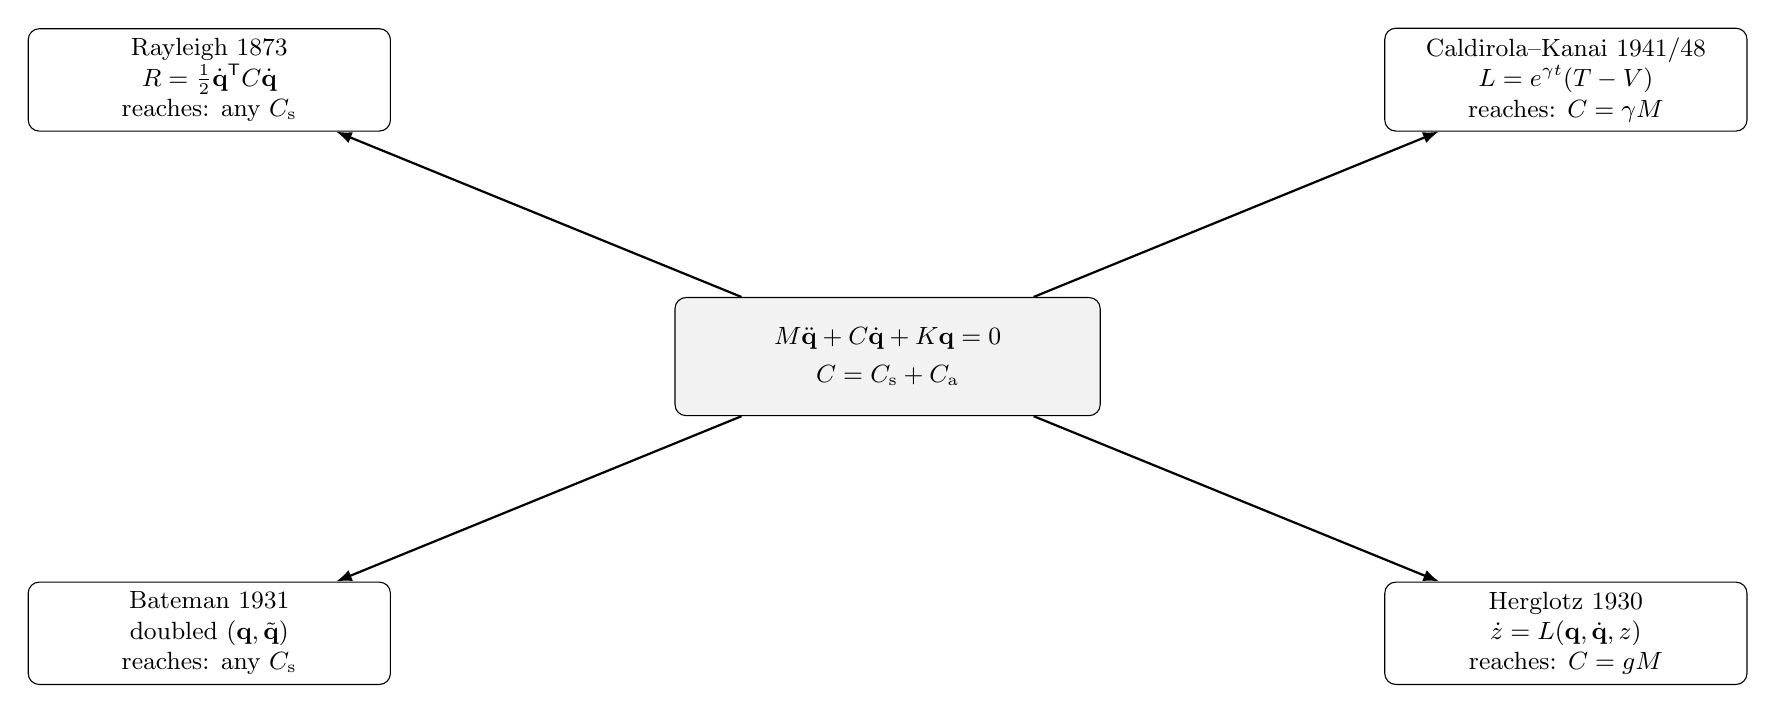
\begin{tikzpicture}[
  node distance=2.1cm and 3.6cm,
  box/.style={draw, rounded corners, align=center, minimum width=4.6cm, minimum height=1.3cm, font=\small},
  center/.style={draw, rounded corners, align=center, minimum width=5.4cm, minimum height=1.5cm, font=\small, fill=gray!10},
  arr/.style={-{Latex[length=2mm]}, thick}
]
  \node[center] (mid) {$\Mm\ddot\vq+\Cc\dot\vq+\Kk\vq=0$\\[1mm] $\Cc=\Cs+\Ca$};
  \node[box, above left=of mid] (ray)  {Rayleigh 1873\\ $R=\tfrac12\dot\vq^{\mathsf T}\Cc\dot\vq$\\ reaches: any $\Cs$};
  \node[box, above right=of mid] (ck)  {Caldirola--Kanai 1941/48\\ $L=e^{\gamma t}(T-V)$\\ reaches: $\Cc=\gamma\Mm$};
  \node[box, below left=of mid] (bat) {Bateman 1931\\ doubled $(\vq,\qt)$\\ reaches: any $\Cs$};
  \node[box, below right=of mid] (her) {Herglotz 1930\\ $\dot z=L(\vq,\dot\vq,z)$\\ reaches: $\Cc=g\Mm$};
  \draw[arr] (mid) -- (ray);
  \draw[arr] (mid) -- (ck);
  \draw[arr] (mid) -- (bat);
  \draw[arr] (mid) -- (her);
\end{tikzpicture}%
}
\caption{Four variational routes to the same multidimensional open system, and the class of damping matrices each one reaches.}
\label{fig:routes}
\end{figure}

\subsection*{Worked example: two dashpots are (generically) not a Caldirola--Kanai system}

Take two unit-free masses $m_1,m_2$, each tethered to a fixed wall by a spring ($k_1$, $k_2$) and to each other by a coupling spring $k_{12}$, and each damped by its own independent dashpot to the fixed frame (rates $c_1,c_2$, \emph{not} connected to one another). This is about as pedestrian a two-degree-of-freedom dissipative system as one can write down:
\[
\Mm=\begin{pmatrix}m_1&0\\0&m_2\end{pmatrix},\qquad
\Kk=\begin{pmatrix}k_1+k_{12}&-k_{12}\\-k_{12}&k_2+k_{12}\end{pmatrix},\qquad
\Cc=\Cs=\begin{pmatrix}c_1&0\\0&c_2\end{pmatrix}.
\]
Rayleigh's function $R=\tfrac12(c_1\dot q_1^2+c_2\dot q_2^2)$ handles it without comment, and so does the Bateman doubling of \S\ref{sec:bateman}. But is it a Caldirola--Kanai system, i.e.\ can the two dashpots be reduced, by a real linear change of coordinates, to two independent, separately-exponentially-damped normal modes? Proposition~\ref{prop:caughey} says: only if $\Cc\Mm^{-1}\Kk=\Kk\Mm^{-1}\Cc$. A direct computation gives
\[
\Cc\Mm^{-1}\Kk-\Kk\Mm^{-1}\Cc = k_{12}\left(\frac{c_1}{m_1}-\frac{c_2}{m_2}\right)\begin{pmatrix}0&1\\-1&0\end{pmatrix},
\]
which vanishes only when $k_{12}=0$ (no coupling at all, in which case the two masses were never a coupled system to begin with) or when $c_1/m_1=c_2/m_2$ (equal damping-to-mass ratio, a very special tuning). For generic, physically unremarkable choices of two independent dashpots on two coupled masses, the system is \emph{non-classically damped}: no real normal-mode transformation decouples it, no sum of one-dimensional Caldirola--Kanai Lagrangians describes it, and the elegant exponential trick of \S\ref{sec:CK} --- along with the single-variable Herglotz construction of \S\ref{sec:herglotz}, confined as it is to the same $\Cc\propto\Mm$ class by Proposition~\ref{prop:herglotz-structural} --- simply does not apply. Rayleigh's 1873 dissipation function and Bateman's 1931 doubling, which never demanded a commuting, simultaneously-diagonalizable structure in the first place, are the two routes that generalize without qualification.
\begin{thebibliography}{99}

\bibitem{Rayleigh1873} Lord Rayleigh (J.\ W.\ Strutt), ``Some General Theorems Relating to Vibrations,'' \emph{Proc.\ London Math.\ Soc.} \textbf{s1-4} (1873), 357--368.

\bibitem{Rayleigh1877} Lord Rayleigh, \emph{The Theory of Sound}, Vol.\ I (Macmillan, London, 1877; reprinted Dover, New York, 1945).

\bibitem{Onsager1931} L.\ Onsager, ``Reciprocal Relations in Irreversible Processes. I,'' \emph{Phys.\ Rev.} \textbf{37} (1931), 405--426.

\bibitem{Casimir1945} H.\ B.\ G.\ Casimir, ``On Onsager's Principle of Microscopic Reversibility,'' \emph{Rev.\ Mod.\ Phys.} \textbf{17} (1945), 343--350.

\bibitem{Caldirola1941} P.\ Caldirola, ``Forze non conservative nella meccanica quantistica,'' \emph{Nuovo Cimento} \textbf{18} (1941), 393--400.

\bibitem{Kanai1948} E.\ Kanai, ``On the Quantization of the Dissipative Systems,'' \emph{Prog.\ Theor.\ Phys.} \textbf{3} (1948), 440--442.

\bibitem{Caughey1960} T.\ K.\ Caughey, ``Classical Normal Modes in Damped Linear Dynamic Systems,'' \emph{J.\ Appl.\ Mech.} \textbf{27} (1960), 269--271.

\bibitem{CaugheyOKelly1965} T.\ K.\ Caughey and M.\ E.\ J.\ O'Kelly, ``Classical Normal Modes in Damped Linear Dynamic Systems,'' \emph{J.\ Appl.\ Mech.} \textbf{32} (1965), 583--588.

\bibitem{Bateman1931} H.\ Bateman, ``On Dissipative Systems and Related Variational Principles,'' \emph{Phys.\ Rev.} \textbf{38} (1931), 815--819.

\bibitem{Dekker1981} H.\ Dekker, ``Classical and Quantum Mechanics of the Damped Harmonic Oscillator,'' \emph{Phys.\ Rep.} \textbf{80} (1981), 1--112.

\bibitem{Ray1979} J.\ R.\ Ray, ``Lagrangians and Systems They Describe: How Not to Treat Dissipation in Quantum Mechanics,'' \emph{Am.\ J.\ Phys.} \textbf{47} (1979), 626--630.

\bibitem{FeshbachTikochinsky} H.\ Feshbach and Y.\ Tikochinsky, ``Quantization of the Damped Harmonic Oscillator,'' in \emph{A Festschrift for I.\ I.\ Rabi}, Trans.\ N.\ Y.\ Acad.\ Sci.\ Ser.\ II \textbf{38} (1977), 44--53.

\bibitem{Chruscinski2005} D.\ Chru\'sci\'nski, ``Quantum Damped Oscillator II: Bateman's Hamiltonian vs.\ 2D Parabolic Potential Barrier,'' \emph{Ann.\ Phys.} \textbf{321} (2006), 840--853.

\bibitem{Herglotz1930} G.\ Herglotz, \emph{Ber\"uhrungstransformationen}, Lectures at the University of G\"ottingen (1930).

\bibitem{GuentherLectures1996} R.\ B.\ Guenther, J.\ A.\ Gottsch, and C.\ M.\ Guenther, \emph{The Herglotz Lectures on Contact Transformations and Hamiltonian Systems}, Lecture Notes in Nonlinear Analysis Vol.\ 1 (Juliusz Schauder Center, Toru\'n, 1996).

\bibitem{GeorgievaGuenther2002} B.\ Georgieva and R.\ Guenther, ``First Noether-Type Theorem for the Generalized Variational Principle of Herglotz,'' \emph{Topol.\ Methods Nonlinear Anal.} \textbf{20} (2002), 261--273.

\bibitem{GeorgievaGuentherBodurov2003} B.\ Georgieva, R.\ Guenther, and T.\ Bodurov, ``Generalized Variational Principle of Herglotz for Several Independent Variables. First Noether-Type Theorem,'' \emph{J.\ Math.\ Phys.} \textbf{44} (2003), 3911--3927.

\end{thebibliography}

\end{document}
